%==============================================================================
% Chapitre 48 - Les pressions nominales
%==============================================================================

\section{Introduction}

Lors du tir, la combustion de la poudre produit une grande quantité de gaz.

Ces gaz exercent une pression sur les parois de l'étui, sur la chambre de
l'arme et sur la base du projectile.

Cette pression constitue la source de l'énergie mécanique permettant
l'accélération du projectile.

\begin{aretenir}

La pression est le principal moteur du mouvement du projectile dans le canon.

\end{aretenir}

\section{Qu'est-ce qu'une pression ?}

La pression correspond à une force appliquée sur une surface.

Elle est définie par la relation :

\begin{equation}
P=\frac{F}{S}
\end{equation}

où :

\begin{itemize}
    \item $P$ représente la pression ;
    \item $F$ représente la force ;
    \item $S$ représente la surface.
\end{itemize}

L'unité internationale de pression est le pascal (Pa).

\section{Ordres de grandeur}

Dans la vie courante, les pressions rencontrées sont relativement faibles.

Par exemple :

\begin{itemize}
    \item pression atmosphérique : environ 101 kPa ;
    \item pression d'un pneu automobile : quelques centaines de kPa.
\end{itemize}

Dans une arme à feu, les pressions atteintes sont considérablement plus
élevées.

\section{Pression dans une cartouche}

Lors de la combustion de la poudre :

\begin{itemize}
    \item des gaz sont produits ;
    \item leur température augmente fortement ;
    \item leur volume tend à augmenter ;
    \item la pression s'élève rapidement.
\end{itemize}

Cette augmentation se produit en quelques millisecondes.

\begin{figure}[htbp]
\centering

\begin{tikzpicture}[scale=1]

\draw[->] (0,0) -- (8,0)
node[right] {Temps};

\draw[->] (0,0) -- (0,5)
node[above] {Pression};

\draw[thick]
(0,0)
.. controls (1,4.5) and (2,5) ..
(3,4)
.. controls (5,2.5) and (6.5,1) ..
(8,0.3);

\node at (2.5,4.8)
{$P_{\max}$};

\end{tikzpicture}

\caption{Évolution simplifiée de la pression au cours d'un tir.}
\label{fig:pression_tir}

\end{figure}

\begin{figure}[htbp]
\centering

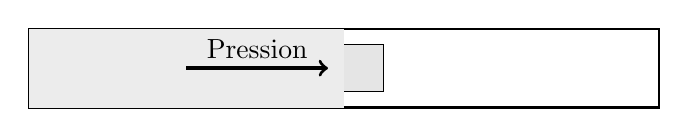
\begin{tikzpicture}[scale=1]

% Canon
\draw[thick] (0,0) rectangle (8,1);

% Projectile
\draw[fill=gray!20]
(4,0.2)
rectangle
(4.5,0.8);

% Gaz
\fill[gray!15]
(0,0)
rectangle
(4,1);

% Force
\draw[->,very thick]
(2,0.5)
--
(3.8,0.5);

\node[above]
at (2.9,0.5)
{Pression};

\end{tikzpicture}

\caption{La pression des gaz exerce une force sur le projectile.}
\label{fig:pression_projectile}

\end{figure}

\section{Pression maximale}

La pression n'est pas constante durant le tir.

Elle augmente rapidement jusqu'à atteindre une valeur maximale.

Cette valeur est souvent appelée :

\begin{quote}
pression maximale admissible
\end{quote}

ou :

\begin{quote}
pression de service maximale.
\end{quote}

\section{Pourquoi limiter la pression ?}

Les armes possèdent des limites mécaniques.

Une pression excessive peut entraîner :

\begin{itemize}
    \item une détérioration de l'arme ;
    \item une rupture de composants ;
    \item des blessures pour le tireur ;
    \item des dommages matériels.
\end{itemize}

La maîtrise de la pression constitue donc un enjeu majeur.

\section{Normalisation}

Les cartouches modernes sont soumises à des normes précises.

Ces normes définissent notamment :

\begin{itemize}
    \item les dimensions ;
    \item les méthodes de mesure ;
    \item les pressions maximales admissibles.
\end{itemize}

Elles garantissent la sécurité et l'interchangeabilité.

\section{La CIP}

En Europe, les pressions sont principalement normalisées par la CIP.

La CIP définit notamment :

\begin{itemize}
    \item les dimensions des chambres ;
    \item les dimensions des cartouches ;
    \item les pressions maximales ;
    \item les procédures d'épreuve.
\end{itemize}

\section{La SAAMI}

Aux États-Unis, un rôle comparable est assuré par la SAAMI.

Cette organisation publie également :

\begin{itemize}
    \item des dimensions ;
    \item des limites de pression ;
    \item des procédures d'essai.
\end{itemize}

\section{Exemples de pressions}

Quelques exemples illustrent les ordres de grandeur rencontrés :

\begin{center}
\begin{tabular}{lc}
\hline
Cartouche & Pression maximale typique \\
\hline
.22 LR & $\approx$ 170 MPa \\
9×19 mm & $\approx$ 235 MPa \\
5,56×45 mm & $\approx$ 430 MPa \\
7,62×51 mm & $\approx$ 415 MPa \\
\hline
\end{tabular}
\end{center}

Les valeurs exactes dépendent des normes utilisées.

\section{Pression et calibre}

Contrairement à une idée répandue, le calibre ne détermine pas à lui seul la
pression.

Deux cartouches de même calibre peuvent fonctionner à des pressions très
différentes.

\section{Pression et vitesse}

Une pression plus élevée permet généralement :

\begin{itemize}
    \item une accélération plus importante ;
    \item une vitesse initiale plus élevée ;
    \item une énergie cinétique plus importante.
\end{itemize}

Cependant, la relation n'est pas strictement proportionnelle.

\section{Pression et longueur de canon}

La pression évolue tout au long du déplacement du projectile.

Elle dépend notamment :

\begin{itemize}
    \item de la combustion de la poudre ;
    \item du volume disponible ;
    \item de la position du projectile.
\end{itemize}

Nous étudierons ces phénomènes en détail dans la partie consacrée à la
balistique intérieure.

\section{Surpression}

On parle de surpression lorsque les limites prévues sont dépassées.

Les causes possibles incluent :

\begin{itemize}
    \item une erreur de chargement ;
    \item une poudre inadaptée ;
    \item un projectile incorrect ;
    \item un enfoncement excessif ;
    \item une obstruction du canon.
\end{itemize}

\section{Sous-pression}

Une pression insuffisante peut également poser problème.

Elle peut provoquer :

\begin{itemize}
    \item un fonctionnement irrégulier ;
    \item une vitesse insuffisante ;
    \item des incidents mécaniques ;
    \item des projectiles bloqués dans le canon.
\end{itemize}

\section{Mesure de la pression}

Les méthodes modernes utilisent généralement :

\begin{itemize}
    \item des capteurs piézoélectriques ;
    \item des équipements instrumentés ;
    \item des bancs d'essai spécialisés.
\end{itemize}

Ces mesures permettent de vérifier la conformité des munitions.

\section{Vers la balistique intérieure}

La pression constitue le phénomène central de la balistique intérieure.

Les chapitres suivants nous permettront de comprendre :

\begin{itemize}
    \item comment elle apparaît ;
    \item comment elle évolue ;
    \item comment elle accélère le projectile.
\end{itemize}

\section{À retenir}

\begin{aretenir}

\begin{itemize}
    \item La pression résulte de la combustion de la poudre.
    \item Elle constitue la source de l'accélération du projectile.
    \item Les pressions sont normalisées par des organismes spécialisés.
    \item Une surpression peut être dangereuse.
    \item La compréhension de la pression est essentielle à la balistique
          intérieure.
\end{itemize}

\end{aretenir}
